\documentclass{article}

\usepackage{amsmath,amssymb,stmaryrd}
\usepackage[margin=1in]{geometry}
\usepackage{graphicx}

\usepackage{microtype}
\usepackage{hyperref}
\usepackage{url}
\usepackage{booktabs}
\usepackage{subcaption}
\usepackage{algorithm}
\usepackage{alltt}
\usepackage{svg}
% \usepackage{color}
\usepackage{algpseudocode}
\usepackage{tikz}
\usepackage{amsthm}
% Ensure required font maps are loaded for newpx/newtx fonts
\pdfmapfile{+newtx.map}
\pdfmapfile{+newpx.map}
\usepackage{newpxtext}
\usepackage{listings}
\usepackage[varg,bigdelims]{newpxmath}
% \usepackage[usenames,dvipsnames]{xcolor}

\theoremstyle{definition}
\newtheorem{definition}{Definition}[section]

\usetikzlibrary{
    cd,
    math,
    backgrounds,
    decorations.markings,
    decorations.pathreplacing,
    positioning,
    arrows.meta,
    circuits.logic.US,
    shapes,
    calc,
    fit,
    trees,
    quotes
}
\definecolor{darkblue}{rgb}{0, 0, 0.5}
\hypersetup{colorlinks=true, citecolor=darkblue, linkcolor=darkblue, urlcolor=darkblue}


\newcommand{\tn}{\textnormal}
\newcommand{\inp}[1]{#1^{\tn{in}}}
\newcommand{\outp}[1]{#1^{\tn{out}}}
\newcommand{\upd}[1]{#1^{\tn{upd}}}
\newcommand{\rdt}[1]{#1^{\tn{rdt}}}


\tikzset{
  WD/.style={%everything after equals replaces "oriented WD" in key.
  	label/.style={
    	font=\everymath\expandafter{\the\everymath\scriptstyle},
      inner sep=0pt,
      node distance=2pt and -2pt},
  	label distance=-2pt,
  	every to/.style={draw},
    semithick,
    node distance=\bbx and \bby,
    decoration={markings, mark=at position \stringdecpos with \stringdec},
    bb port length=3pt,
  	bb port sep=1,
		bb inside color=white,
		bb outside color=black,
	 	bbx = .4cm,
		bb min width=.4cm,
	  bby = 2ex,
	  bb penetrate=0,
	  bb rounded corners=2pt,
	  dot size=3pt,
    shell size = 16pt,
   	penetration = 0pt,
    link size = 2pt,
    shell color = blue,
  	shell inside color=\pcolor!20,
 	  shell outside color=\pcolor!50!black,
  	surround sep=2pt,
    ar/.style={postaction={decorate}},
  	execute at begin picture={\tikzset{
  		x=\bbx, y=\bby, 
			circuit logic US, tiny circuit symbols
			}
		}
  },
  beamer/.style={
  	bbx=.4cm,
		bb min width=.4cm,
		bby=6pt,
		bb port length=3pt,
		bb port sep=.5,
  	dot size=1pt,
    shell size = 11pt, %May look big, but this keeps fonts from mattering.
   	penetration = 0pt,
    link size = 1pt,
    shell color = blue,
    surround sep=1pt,
    inner sep=1pt,
    font=\tiny,
    bb inside color=\picolor,
    bb outside color=\pocolor,
	},
	bb standard colors/.style={bb inside color=white, bb outside color=black},
	bb inside color/.store in=\bbicolor,
	bb outside color/.store in=\bbocolor,
  bbx/.store in=\bbx,
  bby/.store in=\bby,
  bb port sep/.store in=\bbportsep,
  bb port length/.store in=\bbportlen,
  bb penetrate/.store in=\bbpenetrate,
  bb min width/.store in=\bbminwidth,
  bb rounded corners/.store in=\bbcorners,
  bb/.code 2 args={%When you see this key, run the code below:
    \pgfmathsetlengthmacro{\bbheight}{\bbportsep * (max(#1,#2)+1) * \bby}
    \pgfkeysalso{
      draw=\bbocolor,
      fill=\bbicolor,
      minimum height=\bbheight,
      minimum width=\bbminwidth,
      outer sep=0pt,
      rounded corners=\bbcorners,
      thick,
      prefix after command={\pgfextra{\let\fixname\tikzlastnode}},
      append after command={\pgfextra{\draw
      	\ifnum #1=0{} \else foreach \i in {1,...,#1} {
        	($(\fixname.north west)!{(2*\i-1)/(2*#1)}!(\fixname.south west)$) +(-\bbportlen,0) coordinate (\fixname_in\i) -- +(\bbpenetrate,0) coordinate (\fixname_in\i')}\fi 
  					%Define the endpoints of tickmarks
        \ifnum #2=0{} \else foreach \i in {1,...,#2} {
        	($(\fixname.north east)!{(2*\i-1)/(2*#2)}!(\fixname.south east)$) +(-
\bbpenetrate,0) coordinate (\fixname_out\i') -- +(\bbportlen,0) coordinate (\fixname_out\i)}\fi;
       }}}
		},
	dot size/.store in=\dotsize,
	dot/.style={
		circle, draw, thick, inner sep=0, fill=black, minimum width=\dotsize
	},
	bb name/.style={
    append after command={
		\pgfextra{\node[anchor=north] at (\fixname.north) {#1};}
		}
	},
  shell size/.store in=\psize,
	penetration/.store in=\penetration,
  spacing/.store in=\spacing,
  link size/.store in=\lsize,
  shell color/.store in=\pcolor,
 	shell inside color/.store in=\picolor,
 	shell outside color/.store in=\pocolor,
 	surround sep/.store in=\ssep,
 	link/.style={
  	circle, 
  	draw=black, 
  	fill=black,
  	inner sep=0pt, 
 		minimum size=\lsize
 	},
  shell/.style={
 		circle, 
 		draw = \pocolor, 
  	fill = \picolor,
  	minimum size = \psize
  },
  func/.style={
  	shell,
		rectangle,
		rounded corners=.5*\psize,
		inner ysep=.125*\psize,
		minimum width=1.125*\psize,
		inner xsep=.25*\psize,
  },
  funcr/.style={
    func,
    rectangle round north west=false, 
		rectangle round south west=false,
  },
  funcl/.style={
    func,
		rectangle round north east=false, 
		rectangle round south east=false,
  },
  funcu/.style={
    func,
		rectangle round south east=false, 
		rectangle round south west=false,
  },
  funcd/.style={
    func,
		rectangle round north east=false, 
		rectangle round north west=false,
  },
  outer shell/.style={
 		ellipse, 
 		draw,
  	inner sep=\ssep,
  	color=gray,
 	},
  intermediate shell/.style={
 		ellipse,
 		dashed, 
  	draw,
  	inner sep=\ssep,
 		color=\pocolor,
 	},
 }

\tikzset{
	oriented WD/.style={%everything after equals replaces "oriented WD" in key.
		every to/.style={out=0,in=180,draw},
    label/.style={
    	font=\everymath\expandafter{\the\everymath\scriptstyle},
      inner sep=0pt,
      node distance=2pt and -2pt},
    semithick,
    node distance=1 and 1,
    decoration={markings, mark=at position \stringdecpos with \stringdec},
    ar/.style={postaction={decorate}},
    execute at begin picture={\tikzset{
    	x=\bbx, y=\bby,
      every fit/.style={inner xsep=\bbx, inner ysep=\bby}}}
    },
    string decoration/.store in=\stringdec,
    string decoration={\arrow{stealth};},
    string decoration pos/.store in=\stringdecpos,
    string decoration pos=.7,
    bbx/.store in=\bbx,
    bbx = 1.5cm,
    bby/.store in=\bby,
    bby = 1.5ex,
    bb port sep/.store in=\bbportsep,
    bb port sep=1.5,
    % bb wire sep/.store in=\bbwiresep,
    % bb wire sep=1.75ex,
    bb port length/.store in=\bbportlen,
    bb port length=4pt,
    bb penetrate/.store in=\bbpenetrate,
    bb penetrate=0,
    bb min width/.store in=\bbminwidth,
    bb min width=1cm,
    bb rounded corners/.store in=\bbcorners,
    bb rounded corners=2pt,
    bb spider/.style={
    	bb port sep=1, bb port length=10pt, bbx=.4cm, bb min width=.4cm, bby=.8ex},
    bb small/.style={
    	bb port sep=1, bb port length=2.5pt, bbx=.4cm, bb min width=.4cm, bby=.7ex},
		bb medium/.style={
			bb port sep=1, bb port length=2.5pt, bbx=.4cm, bb min width=.4cm, bby=.9ex},
    bb/.code 2 args={%When you see this key, run the code below:
    	\pgfmathsetlengthmacro{\bbheight}{\bbportsep * (max(#1,#2)+1) * \bby}
      \pgfkeysalso{draw,minimum height=\bbheight,minimum
       width=\bbminwidth,outer sep=0pt,
         rounded corners=\bbcorners,thick,
         prefix after command={\pgfextra{\let\fixname\tikzlastnode}},
         append after command={\pgfextra{\draw
            \ifnum #1=0{} \else foreach \i in {1,...,#1} {
            	($(\fixname.north west)!{\i/(#1+1)}!(\fixname.south west)$) +(-\bbportlen,0) coordinate (\fixname_in\i) -- +(\bbpenetrate,0) coordinate (\fixname_in\i')}\fi 
  					%Define the endpoints of tickmarks
            \ifnum #2=0{} \else foreach \i in {1,...,#2} {
            	($(\fixname.north east)!{\i/(#2+1)}!(\fixname.south east)$) +(-
\bbpenetrate,0) coordinate (\fixname_out\i') -- +(\bbportlen,0) coordinate (\fixname_out\i)}\fi;
           }}}
		},
			bb name/.style={
     	append after command={
				\pgfextra{\node[anchor=north] at (\fixname.north) {#1};}
			}
		}
  }


\title{Learning Communication, Coalgebraically}
\author{}
\date{}

\begin{document}
\maketitle

\section{The question}

How can two agents learn to communicate?

Imagine a sequential interaction in which each of two players can output messages, but these messages may initially be written in completely different \emph{languages} (or even modalities).
How, in principle, can they bridge this gap and eventually communicate?

One response would be to create some external goal that the two players A and B must mutually achieve and to treat language like any other action to be learned via reinforcement learning. Specifically, a particularly elegant and instrumentally convergent task is that of predicting future observations. 

At this point, there are several modeling choices.
For instance, we could give A access to B's next observation and have A learn to give short messages to B such that B can predict its observations conditional on A's messages (the messages would have to be short or of a different type than the observations to be interesting, because otherwise the message could be a copy of the observations).

\bigskip
\begin{figure}[H]
\begin{center}
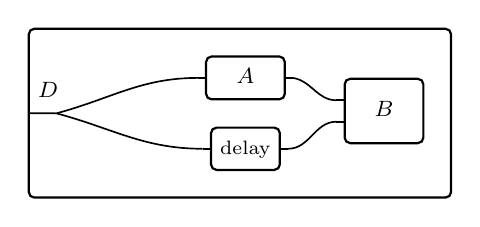
\begin{tikzpicture}
  \begin{scope}[font=\footnotesize, text height=1.5ex, text depth=.5ex]
    \begin{scope}[oriented WD, x=1.6cm, y=.6cm, bb port length=3pt, bb port sep=1.2, dot size=1pt]
    % input, agents, and intermediate blocks
    \node[bb={1}{1}] (A) at (1.5,1) {$A$};
    \node[bb={2}{0}] (B) at (2.6,.3) {$B$};
    \node[bb small, bb={1}{1}] (D1) at (1.5,-0.5) {\scriptsize delay};
    % compute centered split point between A and delayed branch
    \path let \p1=(A_in1), \p2=(D1_in1) in coordinate (SplitA) at (0,{(\y1+\y2)/2});
    % outer box
    \node[bb={0}{0}, fit=(SplitA) (A) (B) (D1), inner sep=10pt] (outer) {};
    % left border wire that splits
    \draw (outer.west) -- node[above,pos=.7] {$D$} (SplitA);
    % wiring per sketch (A feeds top of B) and split to two branches
    \draw (SplitA) to[out=15,in=180] (A_in1);
    \draw (A_out1) to[out=-10,in=180] (B_in1);
    \draw (SplitA) to[out=-15,in=180] (D1_in1);
    \draw (D1_out1) to[out=0,in=180] (B_in2);
  \end{scope}
\end{scope}
\end{tikzpicture}
\end{center}
\caption{Asymmetric sender--receiver setup (counterexample of what we do not want to do). A and B both receive the shared stream $D$, but $A$'s message directly conditions $B$. The upper branch shows $A$'s message feeding into $B$; the lower branch contains one one-step delay block before reaching $B$, ensuring $B$ sees $D$ with a lag so $A$ can comment on the previous observation.}
\end{figure}

\noindent\textit{Exposition.} The outer frame denotes a synchronous system. At each step, both agents receive $D$. Agent $A$ also emits a signal that conditions agent $B$ directly at its top input, while a second copy of $D$ traverses one one-step delay block before entering $B$'s lower input. This lag means that by the time $B$ observes $D$ on the lower branch, $A$ can send a message about the previous observation. Subsequent figures make the messages and learning signals explicit.

\section{Toward a symmetric setup}

But this setup eschews some of the more cooperative/bidirectional/mutually recursive aspects of the genesis of effective communication.
Instead, consider a situation where neither player has privileged information to incoming data; rather, they both have access to a shared input data stream. They each can send messages to the other player, and each player's goal is to maximize the sum of the log probabilities that each player ascribes to their observations, making it a kind of cooperative game.

$$
\lim_{T \to \infty} \frac{1}{T} \sum_{t=1}^{T} \left( \log P_A(\text{observation}_t \mid \text{ctxt}) + \log P_B(\text{observation}_t \mid \text{ctxt}) \right)
$$

\bigskip

\begin{figure}
\begin{center}
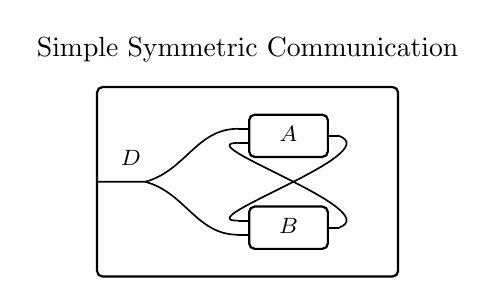
\begin{tikzpicture}
  \begin{scope}[font=\footnotesize, text height=1.5ex, text depth=.5ex]
    \begin{scope}[oriented WD, x=2.6cm, y=.7cm, dot size=1pt, bby=.7ex, bb port sep=1.5]
    % left data tap at frame boundary with explicit split dot
    \node[bb={2}{1}] (A) at (1.6,0.7) {$A$};
    \node[bb={2}{1}, below=.9 of A] (B) {$B$};
    % extra padding to avoid frame hugging contents
    \coordinate (PadL) at (0.8,0);
    \coordinate (PadR) at (2.0,0);
    % expand frame to fit with padding
    \node[bb={0}{0}, fit=(A) (B) (PadL) (PadR), inner sep=10pt] (frameS) {};
    % centered split point vertically (like Fig. 3) at fixed x, not tied to frame border
    \path let \p1=(A_in1), \p2=(B_in2) in coordinate (SplitS) at (0.9,{(\y1+\y2)/2});
    % D originates at left boundary, splits to A(top) and B(bottom)
    \draw (frameS.west) -- node[above,pos=.7] {$D$} (SplitS);
    \draw (SplitS) to[out=15,in=180] (A_in1);
    \draw (SplitS) to[out=-15,in=180] (B_in2);
    % cross messages to remaining inputs
    \draw (A_out1) to[out=-20,in=180] (B_in1);
    \draw (B_out1) to[out=20,in=180] (A_in2);
  \end{scope}
\end{scope}
\node[above=.2cm of frameS.north] {Simple Symmetric Communication};
\end{tikzpicture}
\end{center}
\end{figure}

\section{Players as coalgebras}

We can model each player then as an $F$-coalgebra 
$(S_X,\;\alpha_X\colon S_X\longrightarrow F S_X)$, where $F$ will be specialized to encode the notion that a player can \emph{receive inputs} and \emph{produce outputs} -- e.g. $F(S)\;=\;\mathsf{Out}\times S^{\mathsf{In}}$ for some types $\mathsf{Out}$ and $\mathsf{In}$.

Now we can add in requirements on the structure of $S$, $\mathsf{In}$, and $\mathsf{Out}$ to match the problem setup. First, to model the emergence of communication, we should model the ability of the players to learn. We can do this by expressing $S$ as $\Theta \times \_$, where $\Theta$ is the space of parameterizations of the player's behavior. Next $\mathsf{Out}$ must include A's ``raw'' message type $M_{A\rightarrow B}$. It is ``raw'' because we will need to include some metadata in order to give the learning algorithm the necessary reward signals. 

Next we have $\mathsf{In}_A$ and $\mathsf{In}_B$ which each consist of the other player's output type and the data type $D$ to be predicted: $\mathsf{In}_A=D \times \mathsf{Out}_B$ and $\mathsf{In}_B=D \times \mathsf{Out}_A$.

Then we need a way of talking about the ``probability that a player ascribes to an observation'', and for the learning algorithm to work, we will also need to compute the ``probability of taking a particular action'', where both of these functions are parameterized by $\theta \in \Theta$.
$$
\Theta \xrightarrow{\pi, P} \Delta M \times (\Delta D)^M
$$ where $\pi$ is called the policy, and we require implementations of $\pi$ and $P$ for both players. So the policy produces a distribution over output messages (actions) given a state, and the predictive model $P$ produces a function from messages to distributions over input data.

The state update part of $\alpha$ is going to be a gradient descent step with respect to $\theta \in \Theta$, but the loss function needs to include not only player A's own score $\ln P_\theta^A(d \in D \mid m_{B \rightarrow A})$, but also B's score from the previous round given A's previous message.

So A's state must include not just their weights $\theta_A \in \Theta_A$, but also the score that B received in the previous time step as well as the message that caused that score for the other player.
\section{Prediction and policy components}

Written out, we have $S_A = \Theta_A \times \mathbb{R} \times M_{B\rightarrow A}$ and $S_B = \Theta_B \times \mathbb{R} \times M_{A \rightarrow B}$.
Each player X consists of an initial state $s_0^X$ and functions $U_X : \mathsf{In}_X \times S_X \rightarrow S_X$ and $\Pi_X : S_X \rightarrow \mathsf{Out}_X$, where $\mathsf{Out}_A = M_{A \rightarrow B} \times \mathbb{R} \times M_{B \rightarrow A}$, $\mathsf{In}_A = D \times \mathsf{Out}_B$, and $\mathsf{In}_B = D \times \mathsf{Out}_A$.

Recall we have access to functions $\pi_A : \Theta_A \rightarrow \Delta M_{A \rightarrow B}$, $\pi_B : \Theta_B \rightarrow \Delta M_{B \rightarrow A}$, $P_A : M_{B \rightarrow A} \rightarrow \Delta D$, and $P_B : M_{A \rightarrow B} \rightarrow \Delta D$ to implement $U_A$, $U_B$, $\Pi_A$, and $\Pi_B$.

A natural choice is the following:
\begin{align*}
U_B((d, (m_{A\rightarrow B}, &r_A, m_{B \rightarrow A}^{\text{old}})) : \mathsf{In}_B, (\theta_B, \_, \_) : \Theta_B \times \mathbb{R} \times M_{A \rightarrow B}) : \Theta_B \times \mathbb{R} \times M_{A \rightarrow B} := \\
&\quad (\theta_B - \nabla_{\theta_B} \ln P_{\theta_B} (d \mid m_{A \rightarrow B}) - r_A \nabla_{\theta_B} \pi_{\theta_B} (m_{B \rightarrow A}^{\text{old}}), \ln P_{\theta_B} (d \mid m_{A \rightarrow B}), m_{A \rightarrow B})
\end{align*}

$$\Pi_B((\theta_B, r_B, m_{A \rightarrow B}) : S_B) : M_{B \rightarrow A} \times \mathbb{R} \times M_{A \rightarrow B} := \text{let } m_{B \rightarrow A} \sim \pi_{\theta_B}(\cdot) \text{ in } (m_{B \rightarrow A}, r_B, m_{A \rightarrow B})$$

\begin{figure}
\begin{center}
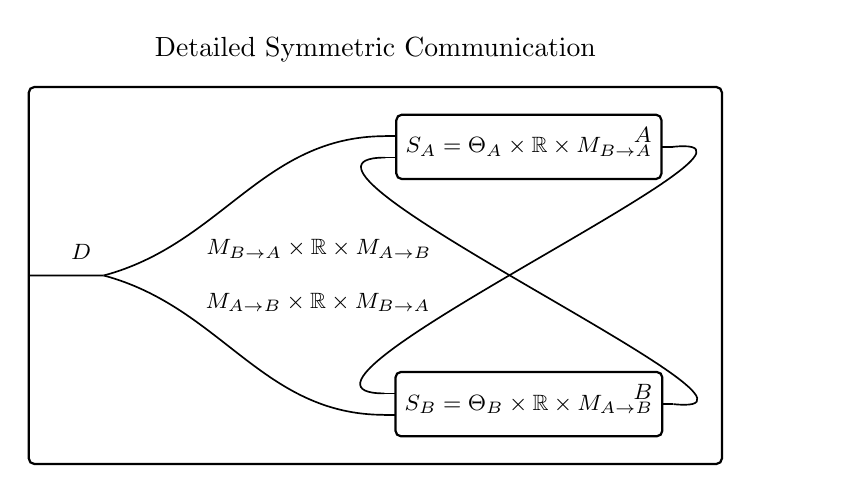
\begin{tikzpicture}
  \begin{scope}[font=\footnotesize, text height=1.5ex, text depth=.5ex]
    \begin{scope}[oriented WD, x=3.0cm, y=.7cm, dot size=1pt, bb port sep=1.2]
    % left data tap with explicit split dot
    \coordinate (Din) at (0,0);
    % agents with state-type labels inside; names at top-right corners
    \node[bb={2}{1}] (A) at (2,1.2) {$S_A=\Theta_A\times\mathbb{R}\times M_{B\to A}$};
    \node[bb={2}{1}, below=3.5 of A] (B) {$S_B=\Theta_B\times\mathbb{R}\times M_{A\to B}$};
    \node[anchor=north east] at (A.north east) {$A$};
    \node[anchor=north east] at (B.north east) {$B$};
    % outer frame with expanded right border
    \coordinate (PadR) at (2.7,0);
    \node[bb={0}{0}, fit=(Din) (A) (B) (PadR), inner sep=10pt] (frame) {};
    % centered split between A_in1 (top) and B_in2 (bottom), moved to the right but keeping y-coordinate centered
    \path let \p1=(A_in1), \p2=(B_in2) in coordinate (SplitD) at (0.2,{(\y1+\y2)/2});
    % D wire from left border to split point, then to A(top) and B(bottom)
    \draw (frame.west) -- node[above,pos=.7] {$D$} (SplitD);
    \draw (SplitD) to[out=15,in=180] (A_in1);
    \draw (SplitD) to[out=-15,in=180] (B_in2);
    % route messages directly; reduce port height and increase separation to avoid collisions
    \tikzset{bby=.6ex, bb port sep=2.2}
    \draw (A_out1) to[out=6,in=180]
      node[pos=.60, left=.1] {$M_{A\to B}\times\mathbb{R}\times M_{B\to A}$}
      (B_in1);
    \draw (B_out1) to[out=-6,in=180]
      node[pos=.60, left=.1] {$M_{B\to A}\times\mathbb{R}\times M_{A\to B}$}
      (A_in2);
  \end{scope}
\end{scope}
\node[above=.2cm of frame.north] {Detailed Symmetric Communication};
\end{tikzpicture}
\end{center}
\end{figure}
The important point is how the weights get updated in $U_A$ / $U_B$.
The $\nabla_{\theta_B} \ln P_{\theta_B}(d \mid m_{A \rightarrow B})$ term allows the player to get better at predicting observations given the other's messages, and $r_A \nabla_{\theta_B} \pi_{\theta_B}(m_{B \rightarrow A})$ is a policy-gradient/REINFORCE-style loss term which is derived from the following observation.
\paragraph{Policy Gradient}
Given system trajectories $\tau$ distributed as $P_\theta(\tau)$, define expected reward

$$
J(\theta)=\mathbb{E}_{\tau\sim P_\theta}[R(\tau)] .
$$

Standard calculus yields

$$
\nabla_\theta J(\theta)
\;=\;
\mathbb{E}_{\tau\sim P_\theta}\!\bigl[R(\tau)\,\nabla_\theta\ln P_\theta(\tau)\bigr].
$$

Here we take

$$
R(\tau)=\frac{1}{n}\sum_{i=1}^{n}\!
\bigl(
\ln P_{\theta_B}(d_i\mid m_{A\to B}^i)
+
\ln P_{\theta_A}(d_i\mid m_{B\to A}^i)
\bigr).
$$

Writing the trajectory as triples
$(d_i,m_{A\to B}^i,m_{B\to A}^i)_{i\ge 0}$,

$$
P_\theta(\tau)
=\prod_{i}
P(d_i)\;
\pi_{\theta_A}(m_{A\to B}^i)
\;
\pi_{\theta_B}(m_{B\to A}^i),
$$

with
$\theta_A^{i+1}=U_A(d_i,m_{B\to A}^i,\theta_A^i)$
and likewise for~$\theta_B$.

Hence

$$
\nabla_{\theta_A}\ln P_\theta(\tau)
=\sum_{i}\nabla_{\theta_A}\ln\pi_{\theta_A}(m_{A\to B}^i).
$$

\section{Possible improvements}\label{sec:improvements}

So currently, our online learning algorithm would be quite high variance, and it might help us to modify the setup to:
\begin{enumerate}
\item remember more previous messages and rewards so we could better approximate $\sum_{i=0}^{\infty} \gamma^i r_i$, the return of the trajectory, and 
\item add ``batching'' into the type signature so we can use GRPO-style averaging to decrease the variance of the estimator.
\end{enumerate}

I would also like to derive our update function from something closer to first principles, e.g., deriving $U$ by maximizing the probability of the trajectory with respect to $U$.

\end{document}

